Lorem ipsum dolor sit amet, consectetur adipisicing elit, sed do eiusmod
tempor incididunt ut labore et dolore magna aliqua. Ut enim ad minim veniam,
quis nostrud exercitation ullamco laboris nisi ut aliquip ex ea commodo
consequat. Duis aute irure dolor in reprehenderit in voluptate velit esse
cillum dolore eu fugiat nulla pariatur. Excepteur sint occaecat cupidatat non
proident, sunt in culpa qui officia deserunt mollit anim id est laborum.


\begin{figure}
    \centering
    \addletter{140}{a}
    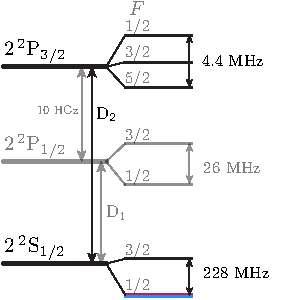
\includegraphics{fig-ai/li-levels-base.pdf}
    \hfill
    \addletter{140}{b}
    \includegraphics{fig-py/li6-zeeman.pdf}
    \hfill
    \addletter{140}{c}
    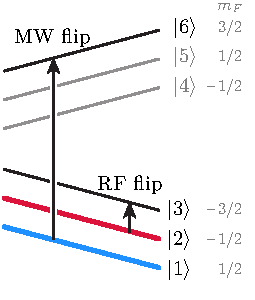
\includegraphics{fig-ai/li-levels.pdf}
    \caption{\textbf{${}^6$Li energy levels}. a) Level diagram of the ground and 2P excited states of ${}^6$Li \cite{gehm_preparation_2003}. b) Zeeman splitting of the hyperfine levels of the $2\, {}^2\mathrm{S}_{1/2}$ state in ${}^6$Li \cite{serwane_deterministic_2011, sibalic_arc_2017}. With dashed line was marked non-interacting regime for 1-2 mixture at 527 Gs. c) As different spin states for physics we consider state $\ket{1}$ and $\ket{2}$, but for imaging it is worth to flip them to close transitions.}
    \label{fig:li6levels}
\end{figure}

Lorem ipsum dolor sit amet, consectetur adipisicing elit, sed do eiusmod
tempor incididunt ut labore et dolore magna aliqua. Ut enim ad minim veniam,
quis nostrud exercitation ullamco laboris nisi ut aliquip ex ea commodo
consequat. Duis aute irure dolor in reprehenderit in voluptate velit esse
cillum dolore eu fugiat nulla pariatur. Excepteur sint occaecat cupidatat non
proident, sunt in culpa qui officia deserunt mollit anim id est laborum.

Добавить, что наблюдали и BEC молекулярный. RF-flip and MW-flip
